\documentclass[14pt]{beamer}
\usetheme{Boadilla}

\makeatother
\setbeamertemplate{footline}

\makeatletter
\setbeamertemplate{navigation symbols}{}
\setbeamertemplate{items}[circle]
\usepackage{tikz}
\usepackage{amsmath}
\usepackage{relsize}
\usepackage{graphics}


\title{Los Angeles Coutny}
\date{\today}
\author{Bryan Wilcox}
\institute{UCLA}

\begin{document}

\begin{frame}
\titlepage
\end{frame}


\begin{frame}{2012 Voter Turnout in Los Angeles County}
\begin{figure}[htb!]
\vskip-1ex
  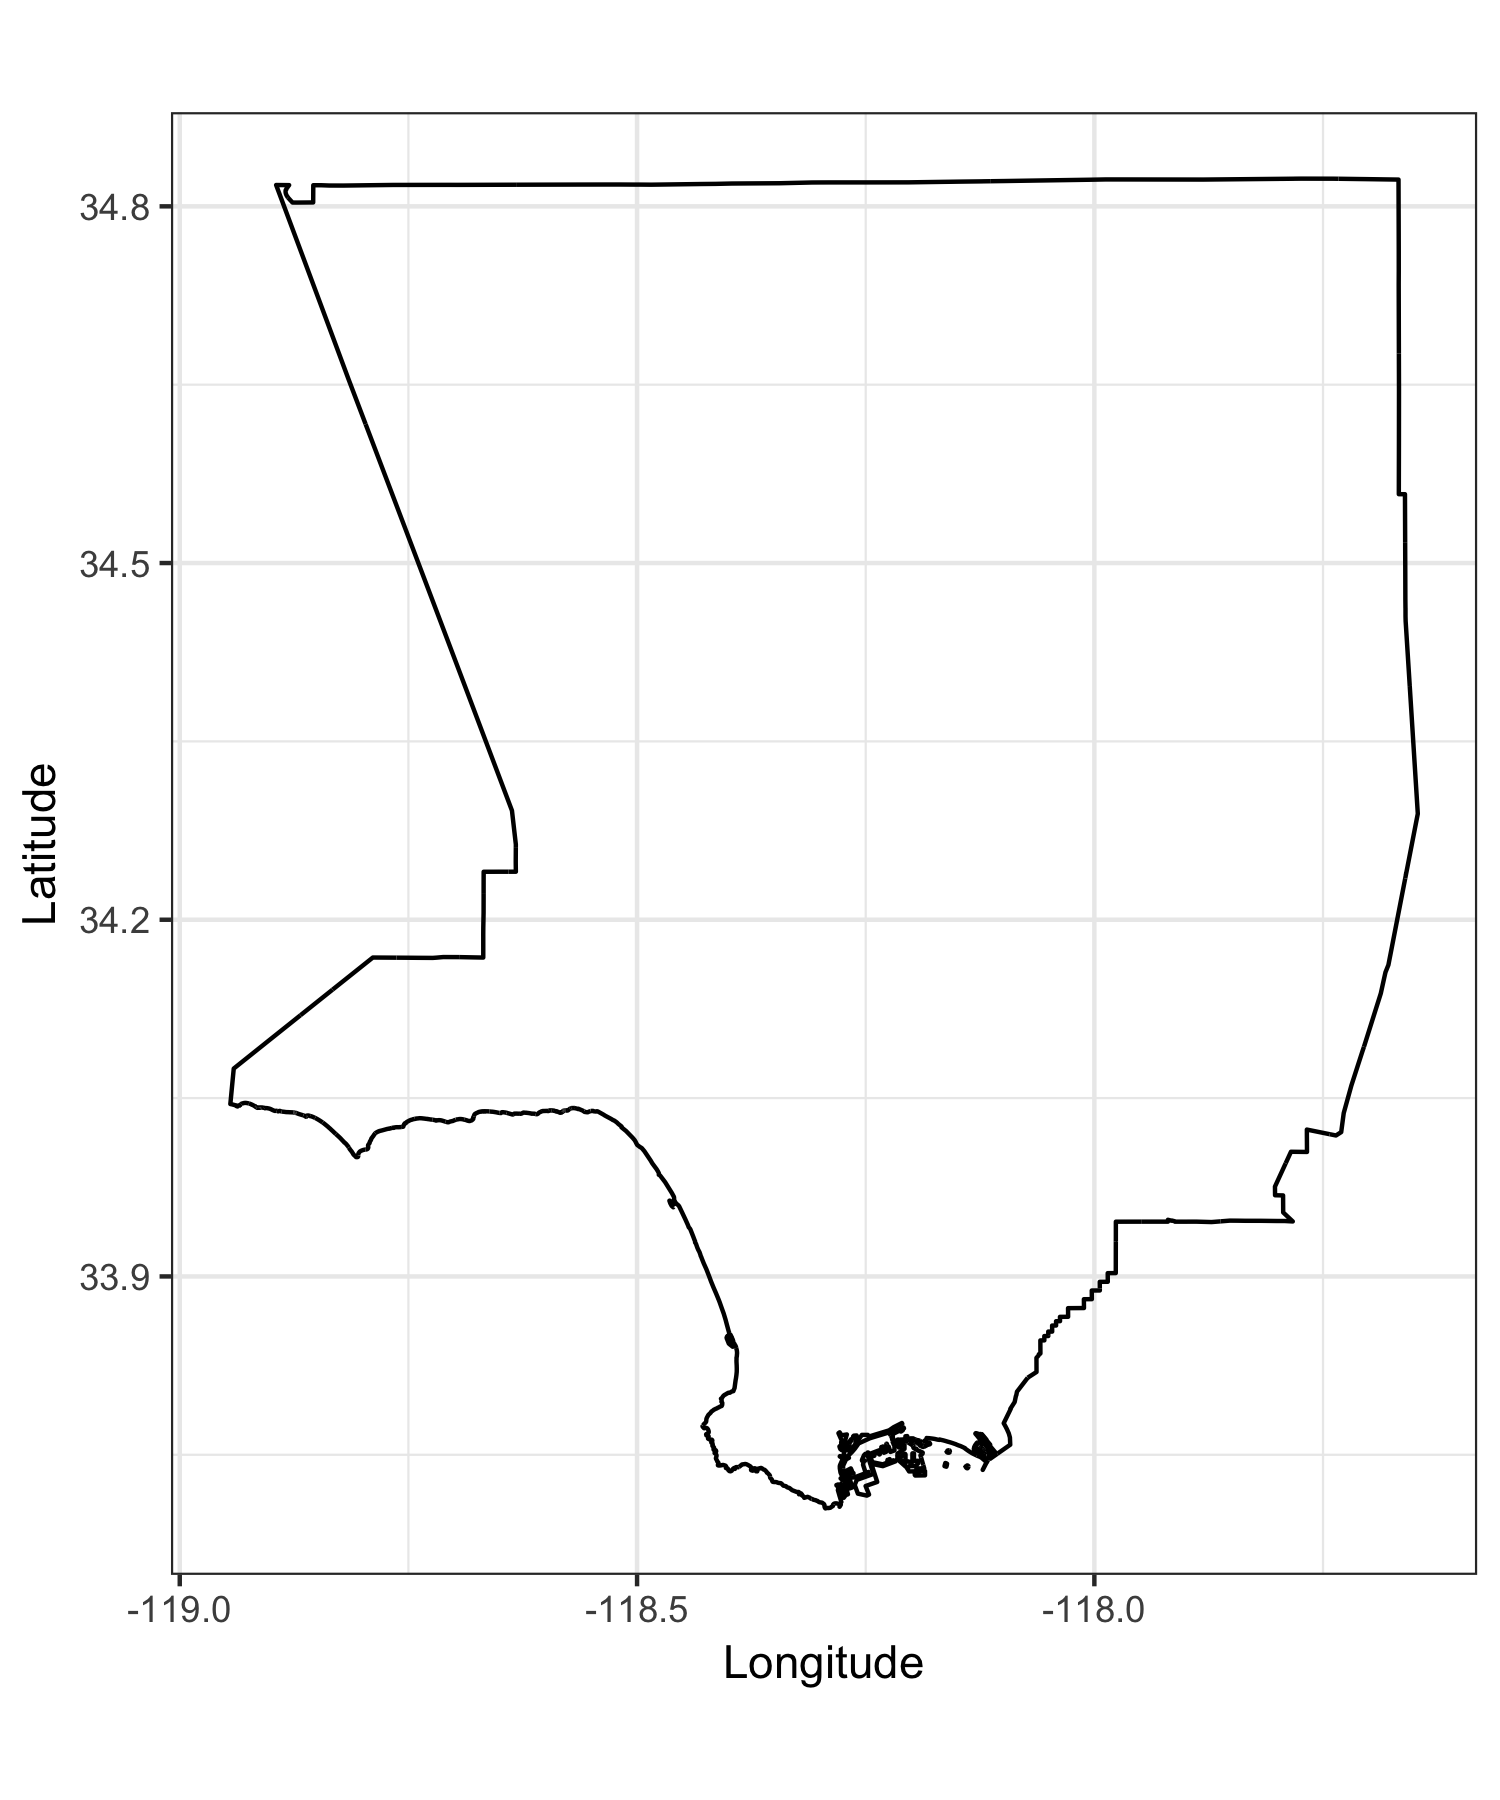
\includegraphics[width=75mm]{/Users/bryanwilcox/Dropbox/Courses/UCLA/2017_winter/stats_273_geostats/stats_273_geo_stats/la_county.png}\\  
%\vskip-6ex
\end{figure} 
\end{frame}


\begin{frame}{Zillow's neighborhoods in LA County}
\begin{figure}[htb!]
\vskip-1ex
  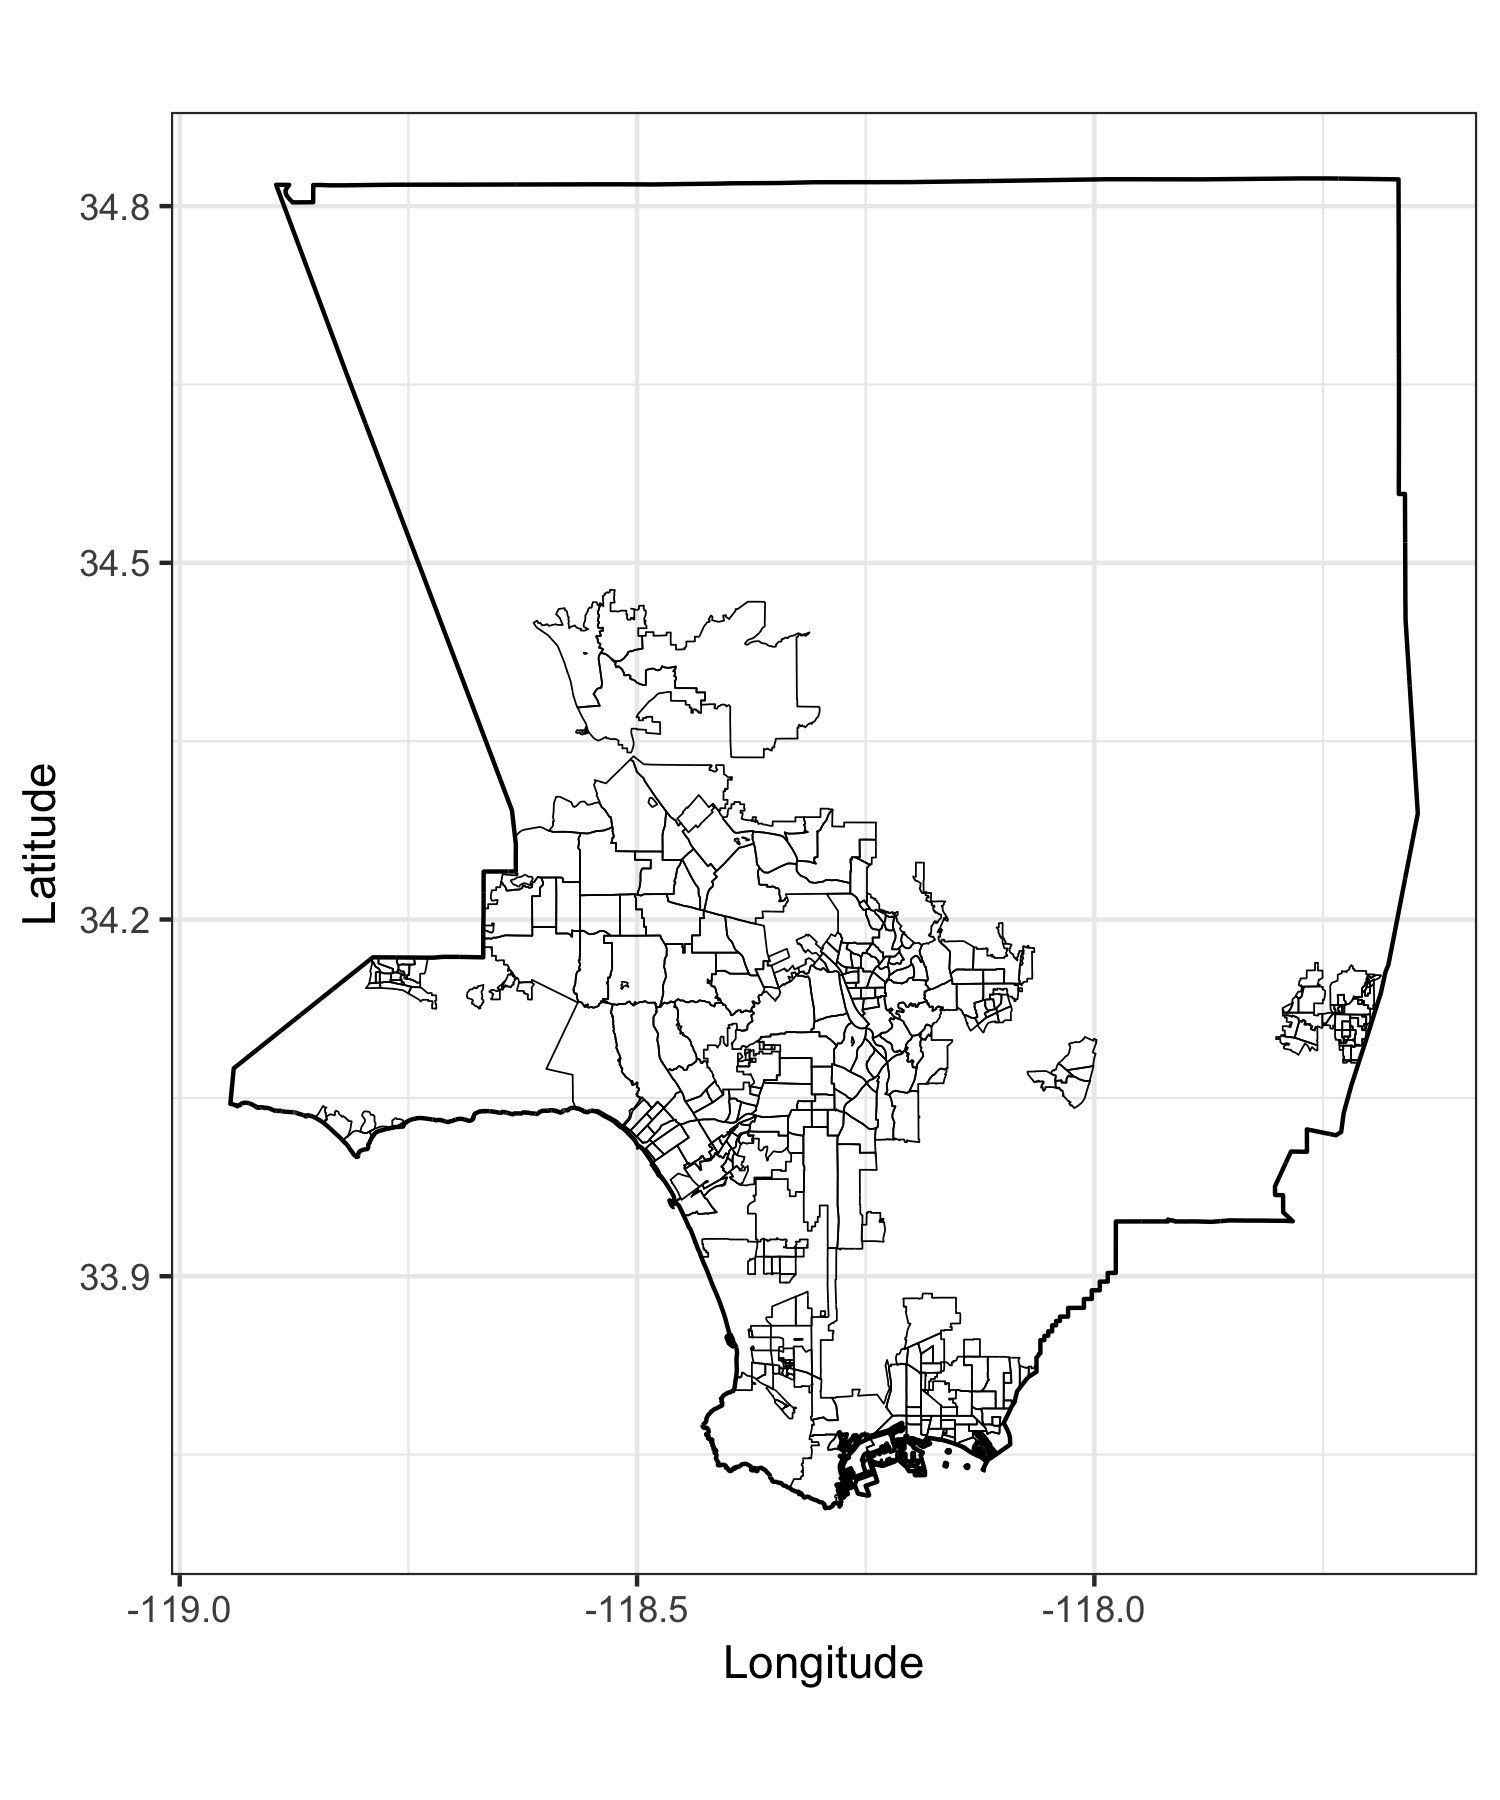
\includegraphics[width=75mm]{/Users/bryanwilcox/Dropbox/Courses/UCLA/2017_winter/stats_273_geostats/stats_273_geo_stats/la_county_hoods.png}\\  
%\vskip-6ex
\end{figure} 
\end{frame}



\begin{frame}{Registered Voters across LA County}
\begin{figure}[htb!]
\vskip-1ex
  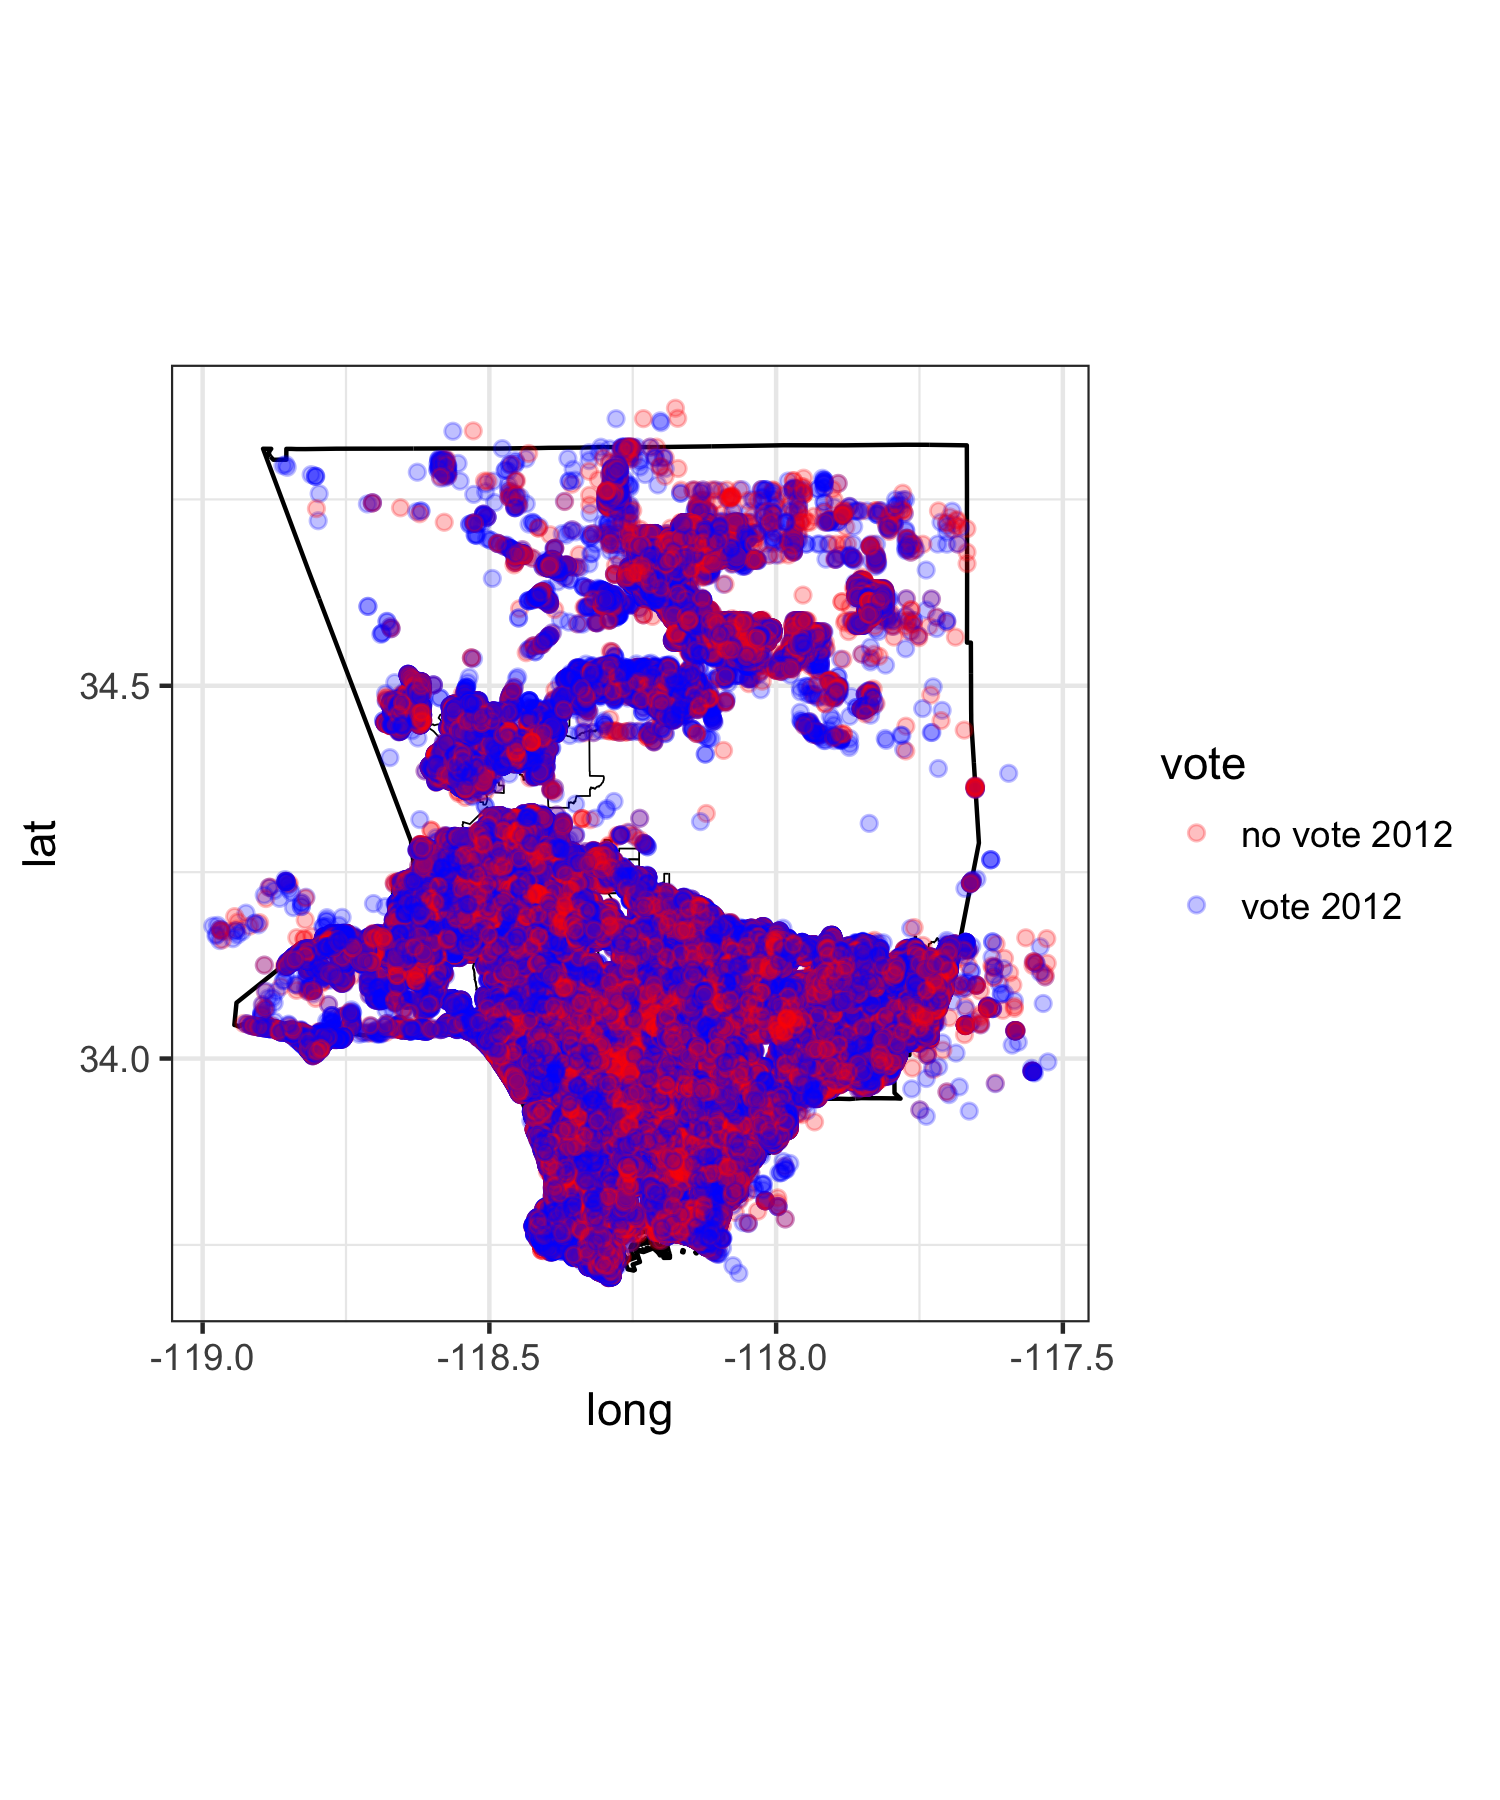
\includegraphics[width=85mm]{/Users/bryanwilcox/Dropbox/Courses/UCLA/2017_winter/stats_273_geostats/stats_273_geo_stats/la_county_voters.png}\\  
%\vskip-6ex
\end{figure} 
\end{frame}

\begin{frame}{Let's look at neighborhood level turnout}
\begin{figure}[htb!]
\vskip-1ex
  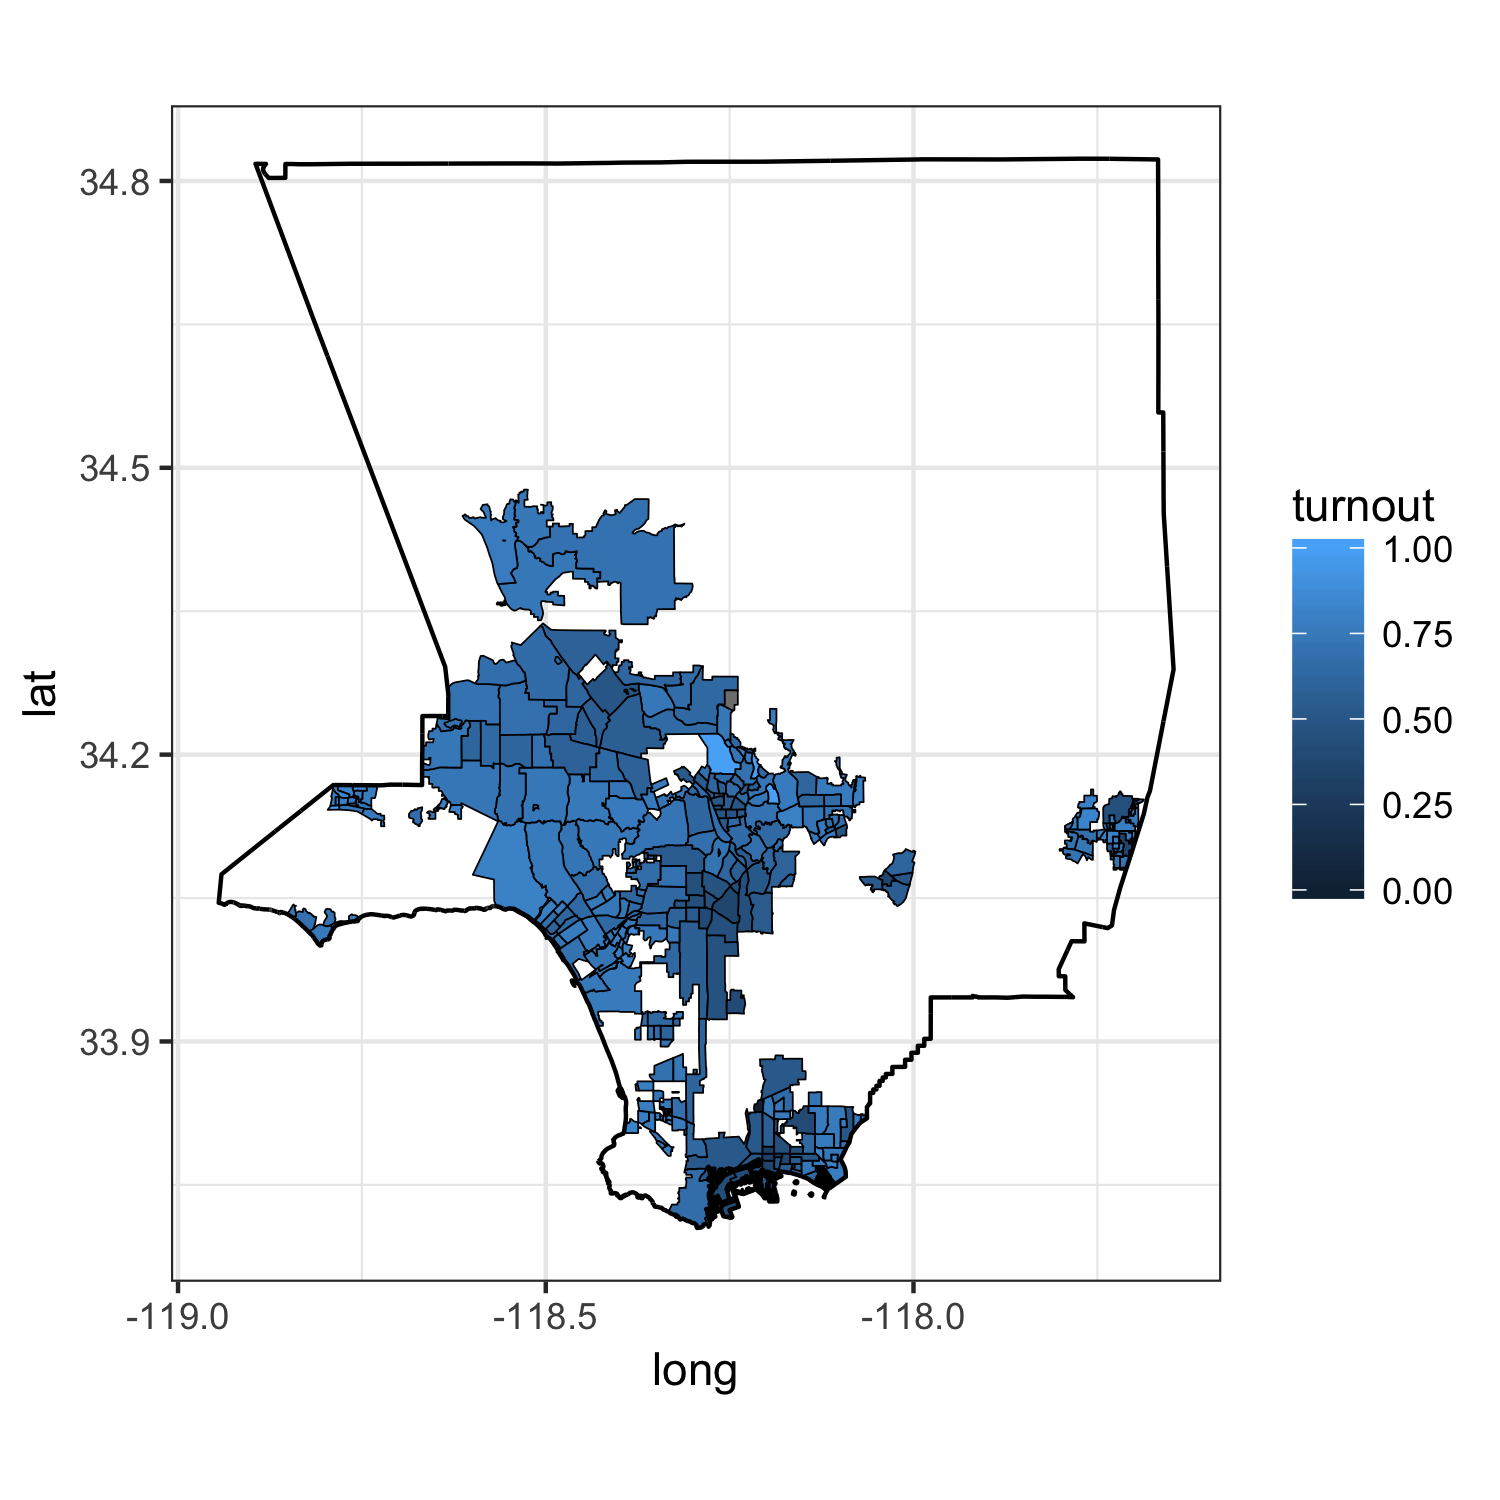
\includegraphics[width=85mm]{/Users/bryanwilcox/Dropbox/Courses/UCLA/2017_winter/stats_273_geostats/stats_273_geo_stats/neighborhood_turnout.png}\\  
%\vskip-6ex
\end{figure} 
\end{frame}

\begin{frame}{The average turnout is across the neighborhoods is 68\%}
\begin{figure}[htb!]
\vskip-1ex
  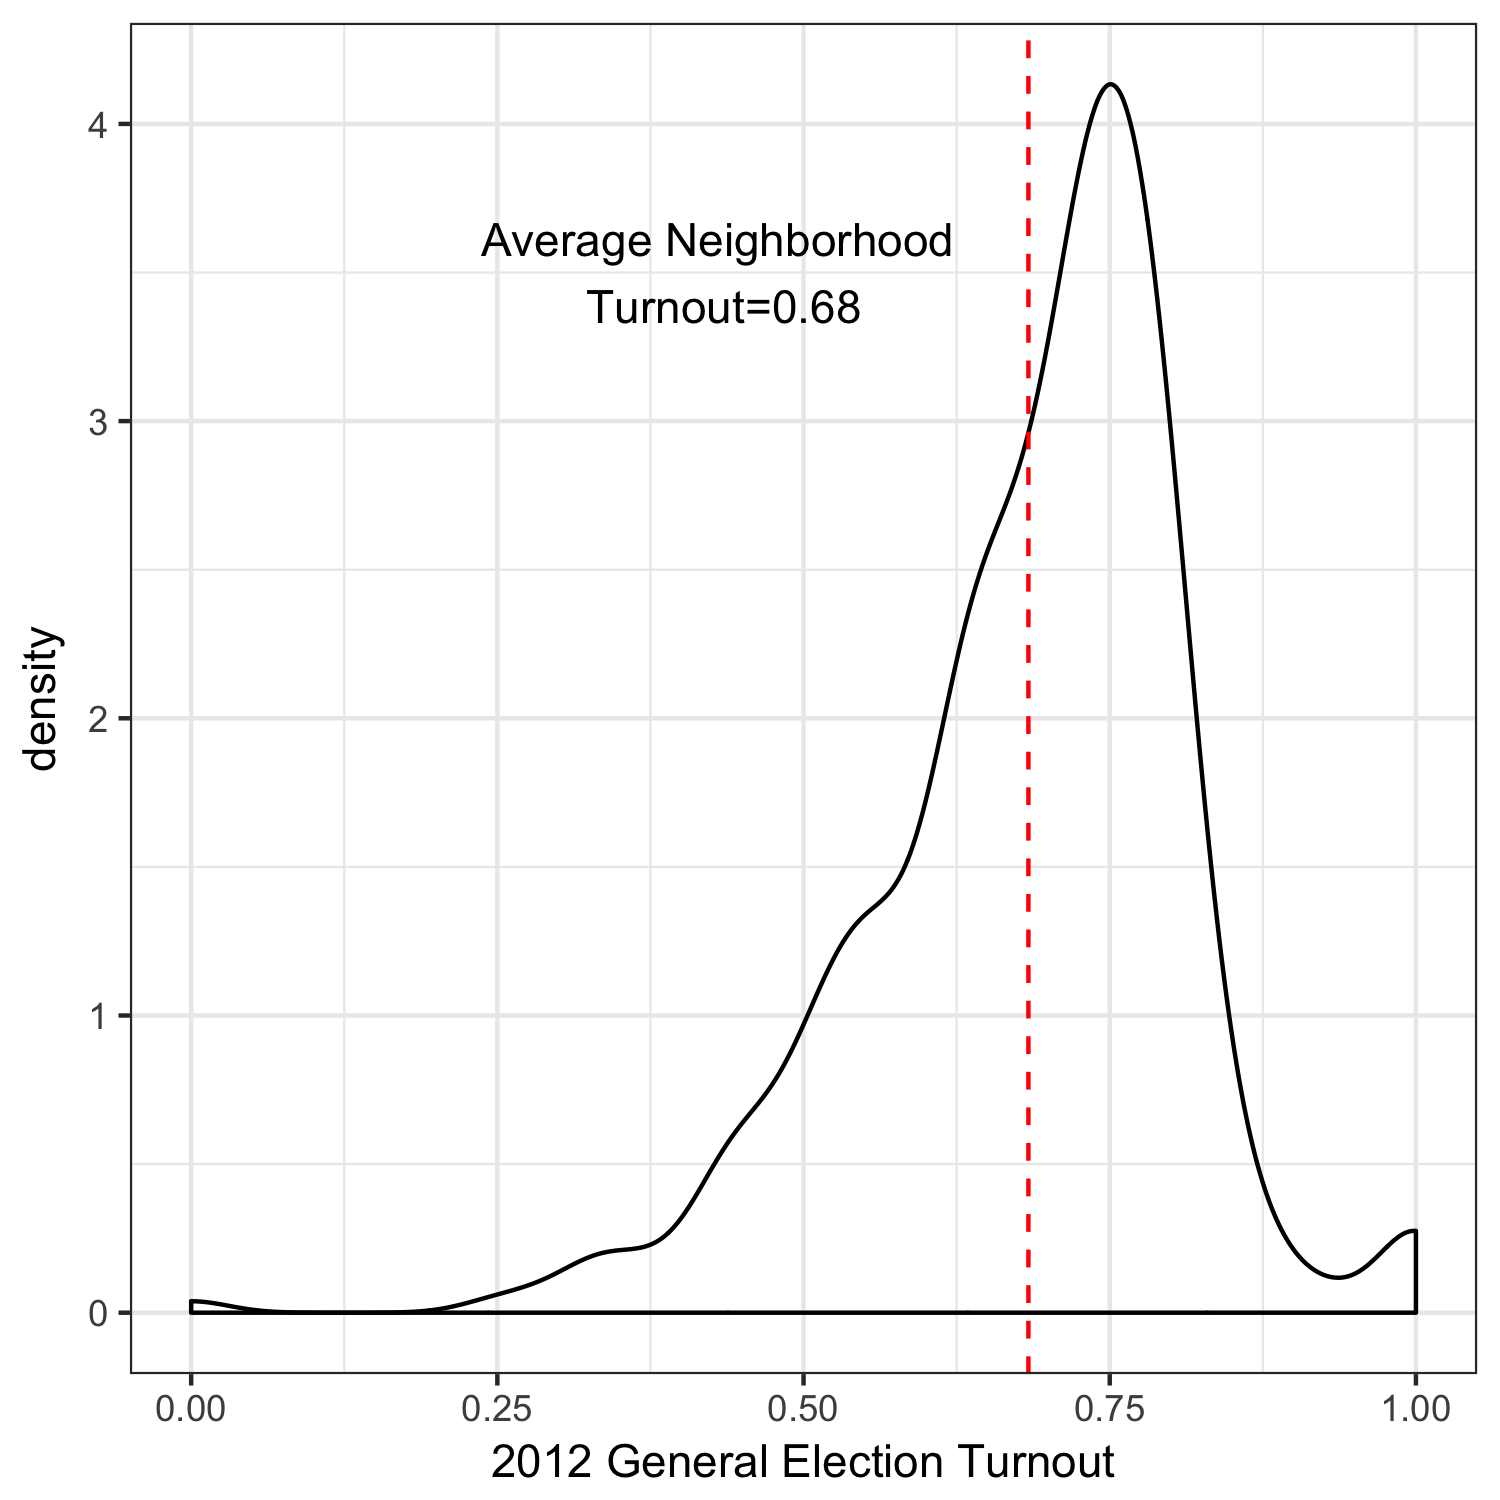
\includegraphics[width=75mm]{/Users/bryanwilcox/Dropbox/Courses/UCLA/2017_winter/stats_273_geostats/stats_273_geo_stats/neighborhood_turnout_density.png}\\  
%\vskip-6ex
\end{figure} 
\end{frame}

\begin{frame}{Here are the neighborhood centroids, which we will use as spatial points}
\begin{figure}[htb!]
\vskip-1ex
  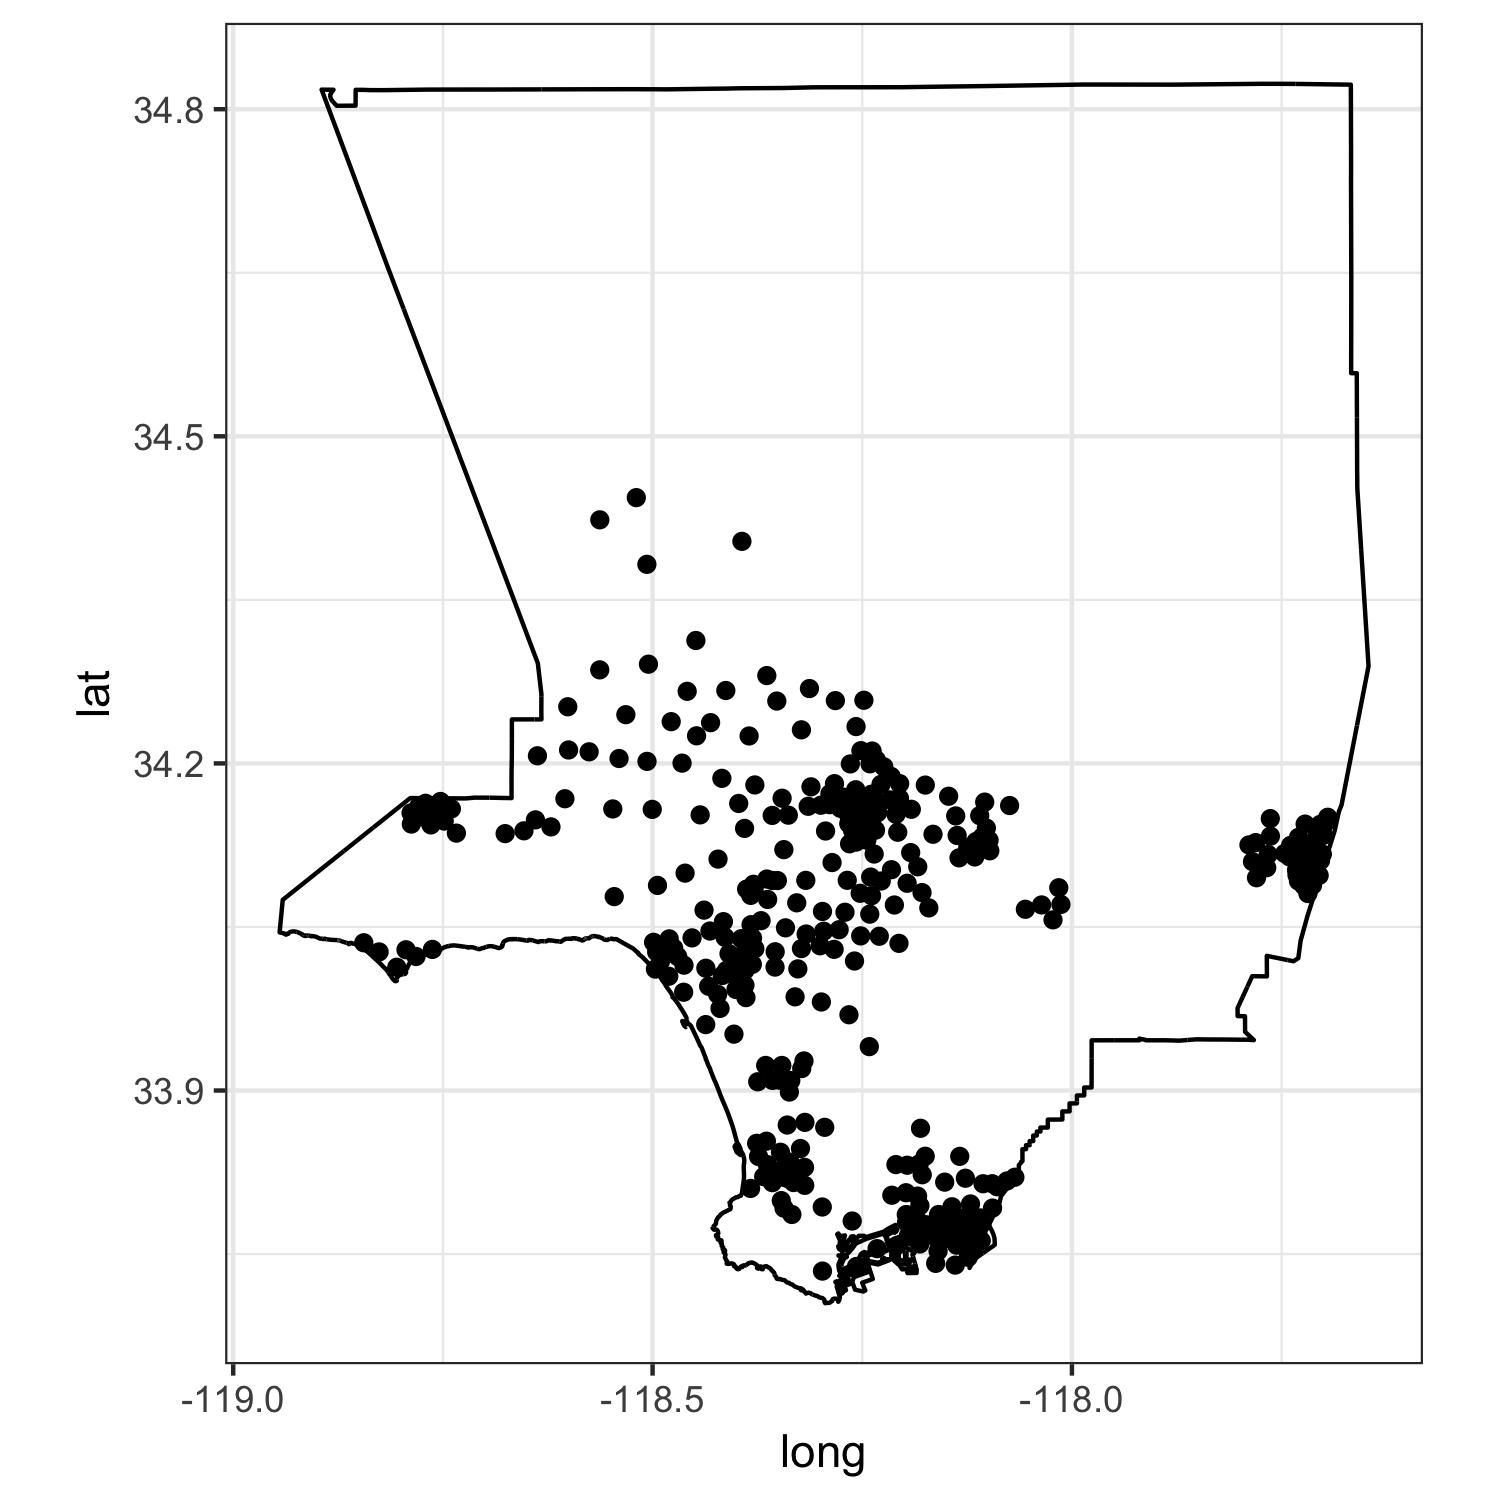
\includegraphics[width=75mm]{/Users/bryanwilcox/Dropbox/Courses/UCLA/2017_winter/stats_273_geostats/stats_273_geo_stats/neighborhood_centroids.png}\\  
%\vskip-6ex
\end{figure} 
\end{frame}

\begin{frame}{Variograms}
\begin{figure}[htb!]
\vskip-1ex
  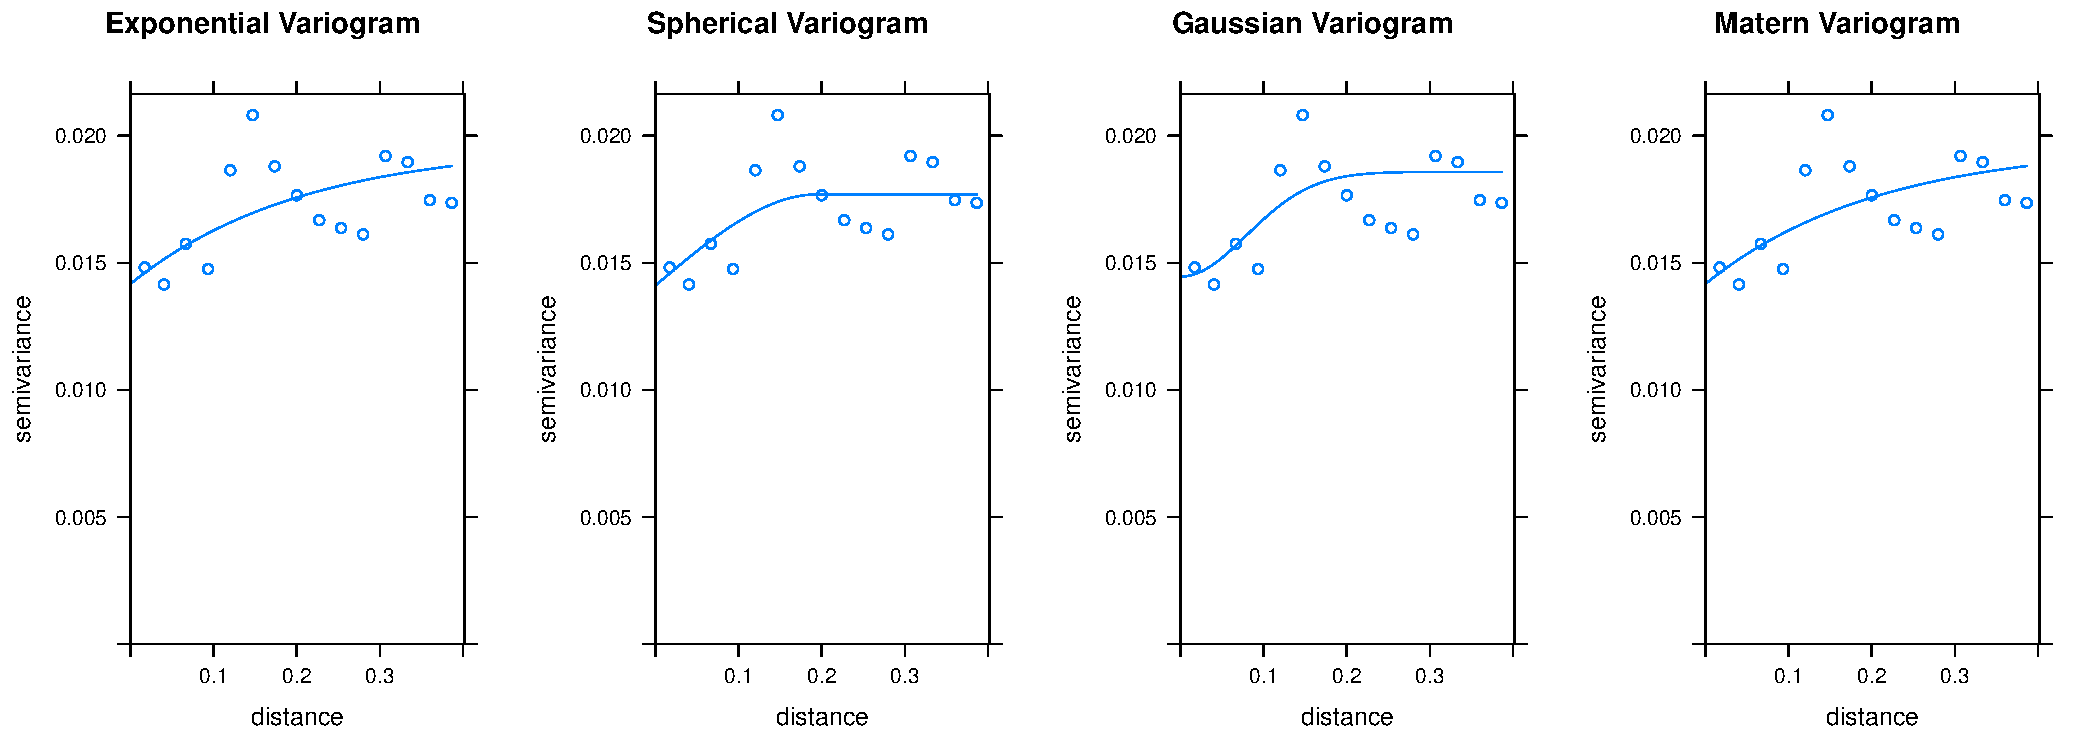
\includegraphics[width=125mm]{/Users/bryanwilcox/Dropbox/Courses/UCLA/2017_winter/stats_273_geostats/stats_273_geo_stats/variogram.pdf}\\  
%\vskip-6ex
\end{figure} 
\end{frame}


\begin{frame}{Cross-validation to select variogram}
\begin{figure}[htb!]
%\caption{Predicted High Linked Fate with Census Data for Blacks} \label{fig:title}
\vskip-1ex
  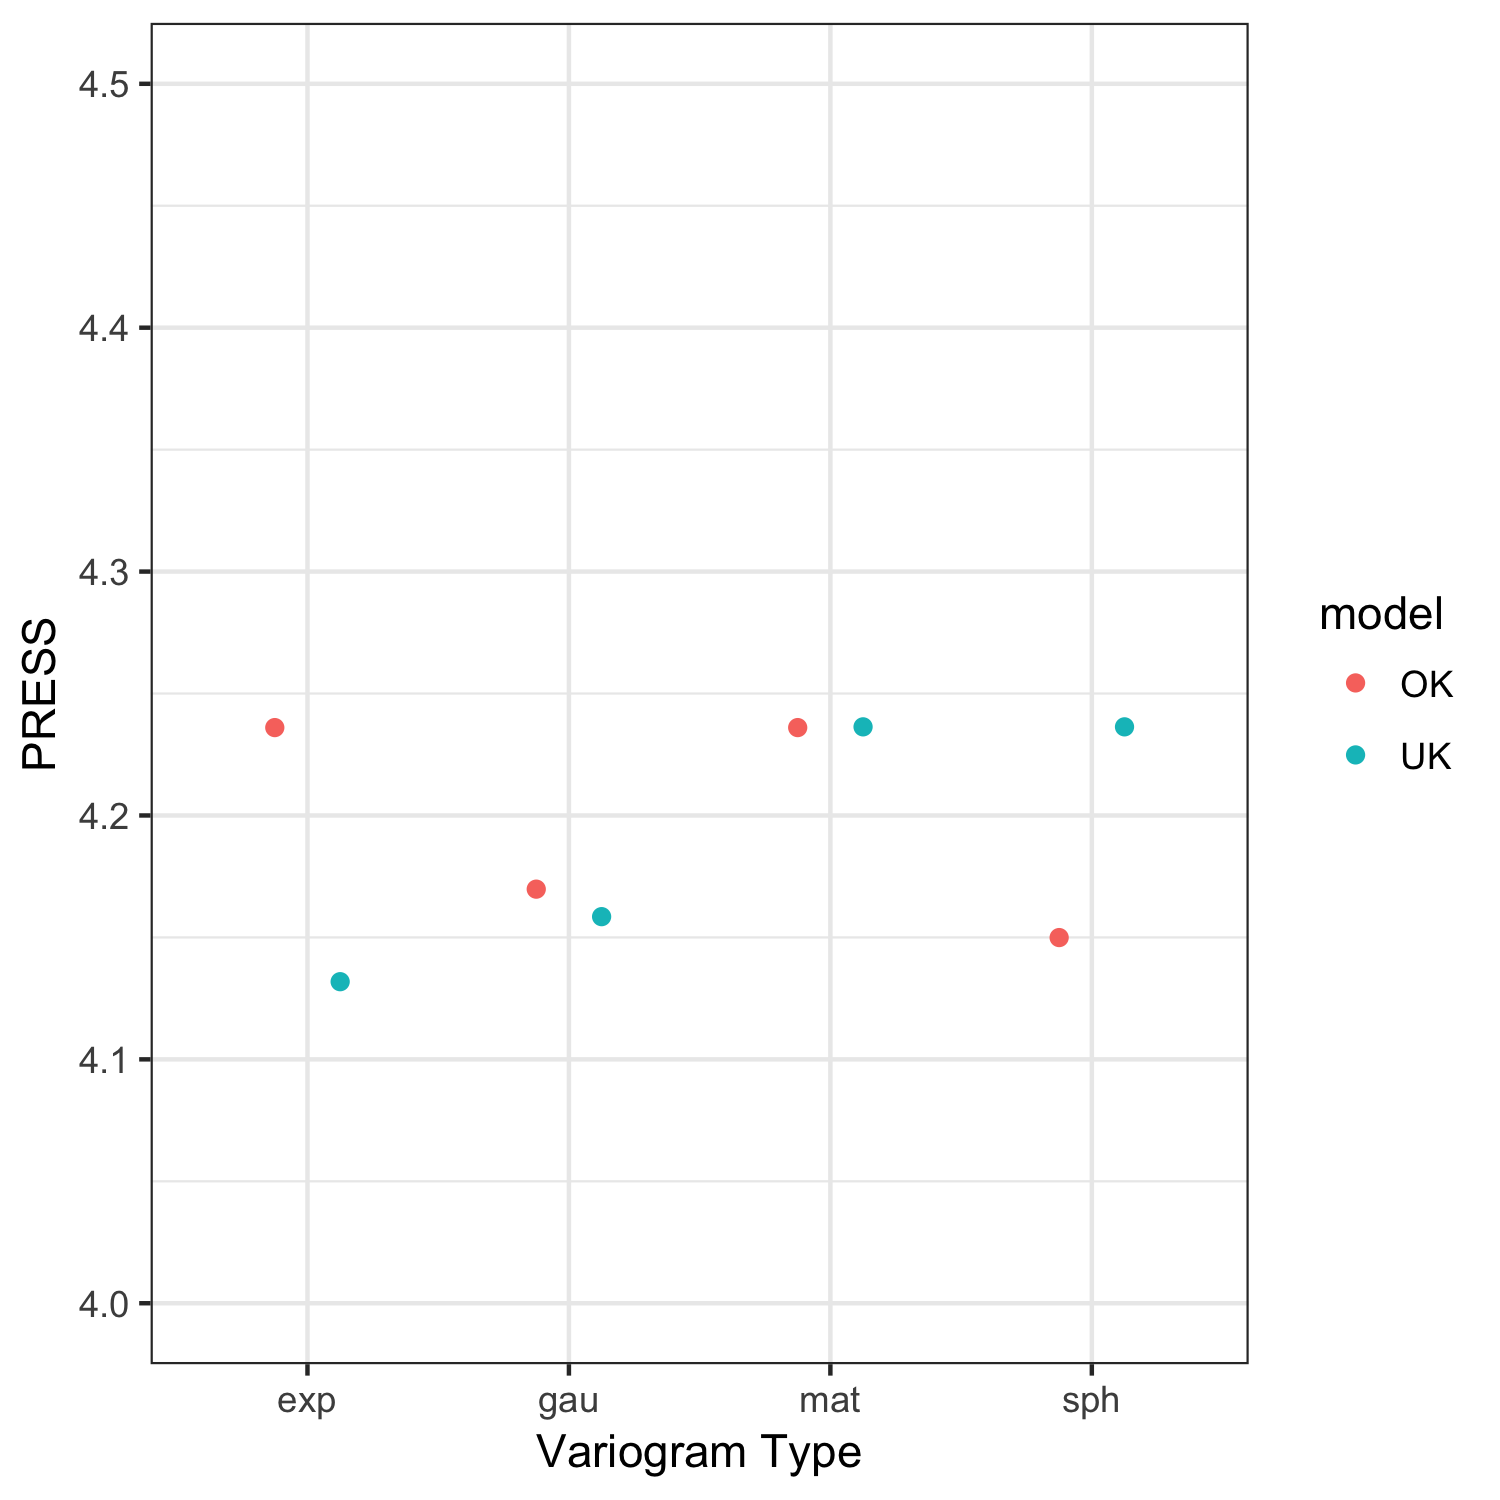
\includegraphics[width=85mm]{/Users/bryanwilcox/Dropbox/Courses/UCLA/2017_winter/stats_273_geostats/stats_273_geo_stats/vg_cv.png}\\  
%\vskip-6ex
\end{figure} 
\end{frame}

\begin{frame}{Ordinary Krigging as Prediction}
\begin{figure}[htb!]
%\caption{Predicted High Linked Fate with Census Data for Blacks} \label{fig:title}
\vskip-1ex
  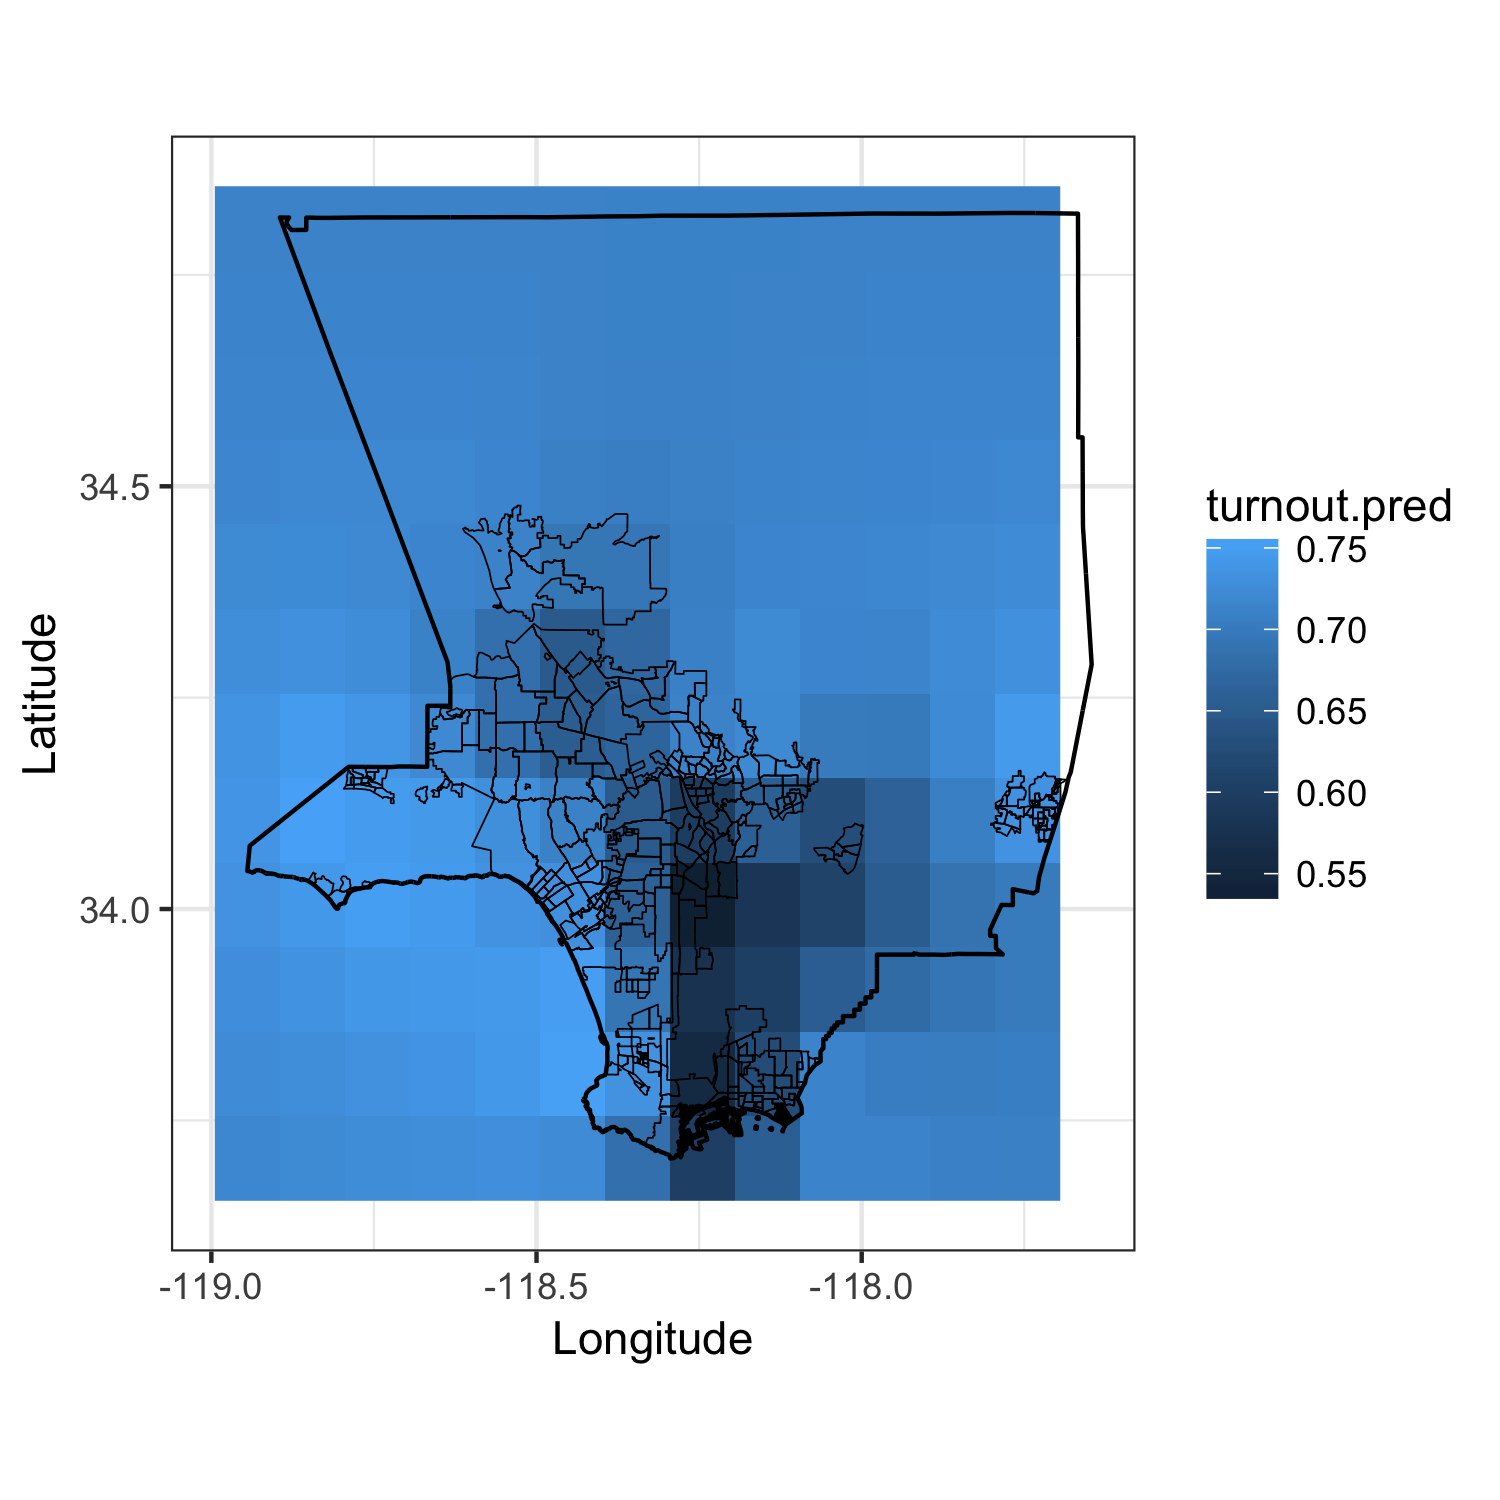
\includegraphics[width=85mm]{/Users/bryanwilcox/Dropbox/Courses/UCLA/2017_winter/stats_273_geostats/stats_273_geo_stats/pred_ok.png}\\  
%\vskip-6ex
\end{figure} 
\end{frame}

\begin{frame}{Universal Krigging as Prediction}
\begin{figure}[htb!]
%\caption{Predicted High Linked Fate with Census Data for Blacks} \label{fig:title}
\vskip-1ex
  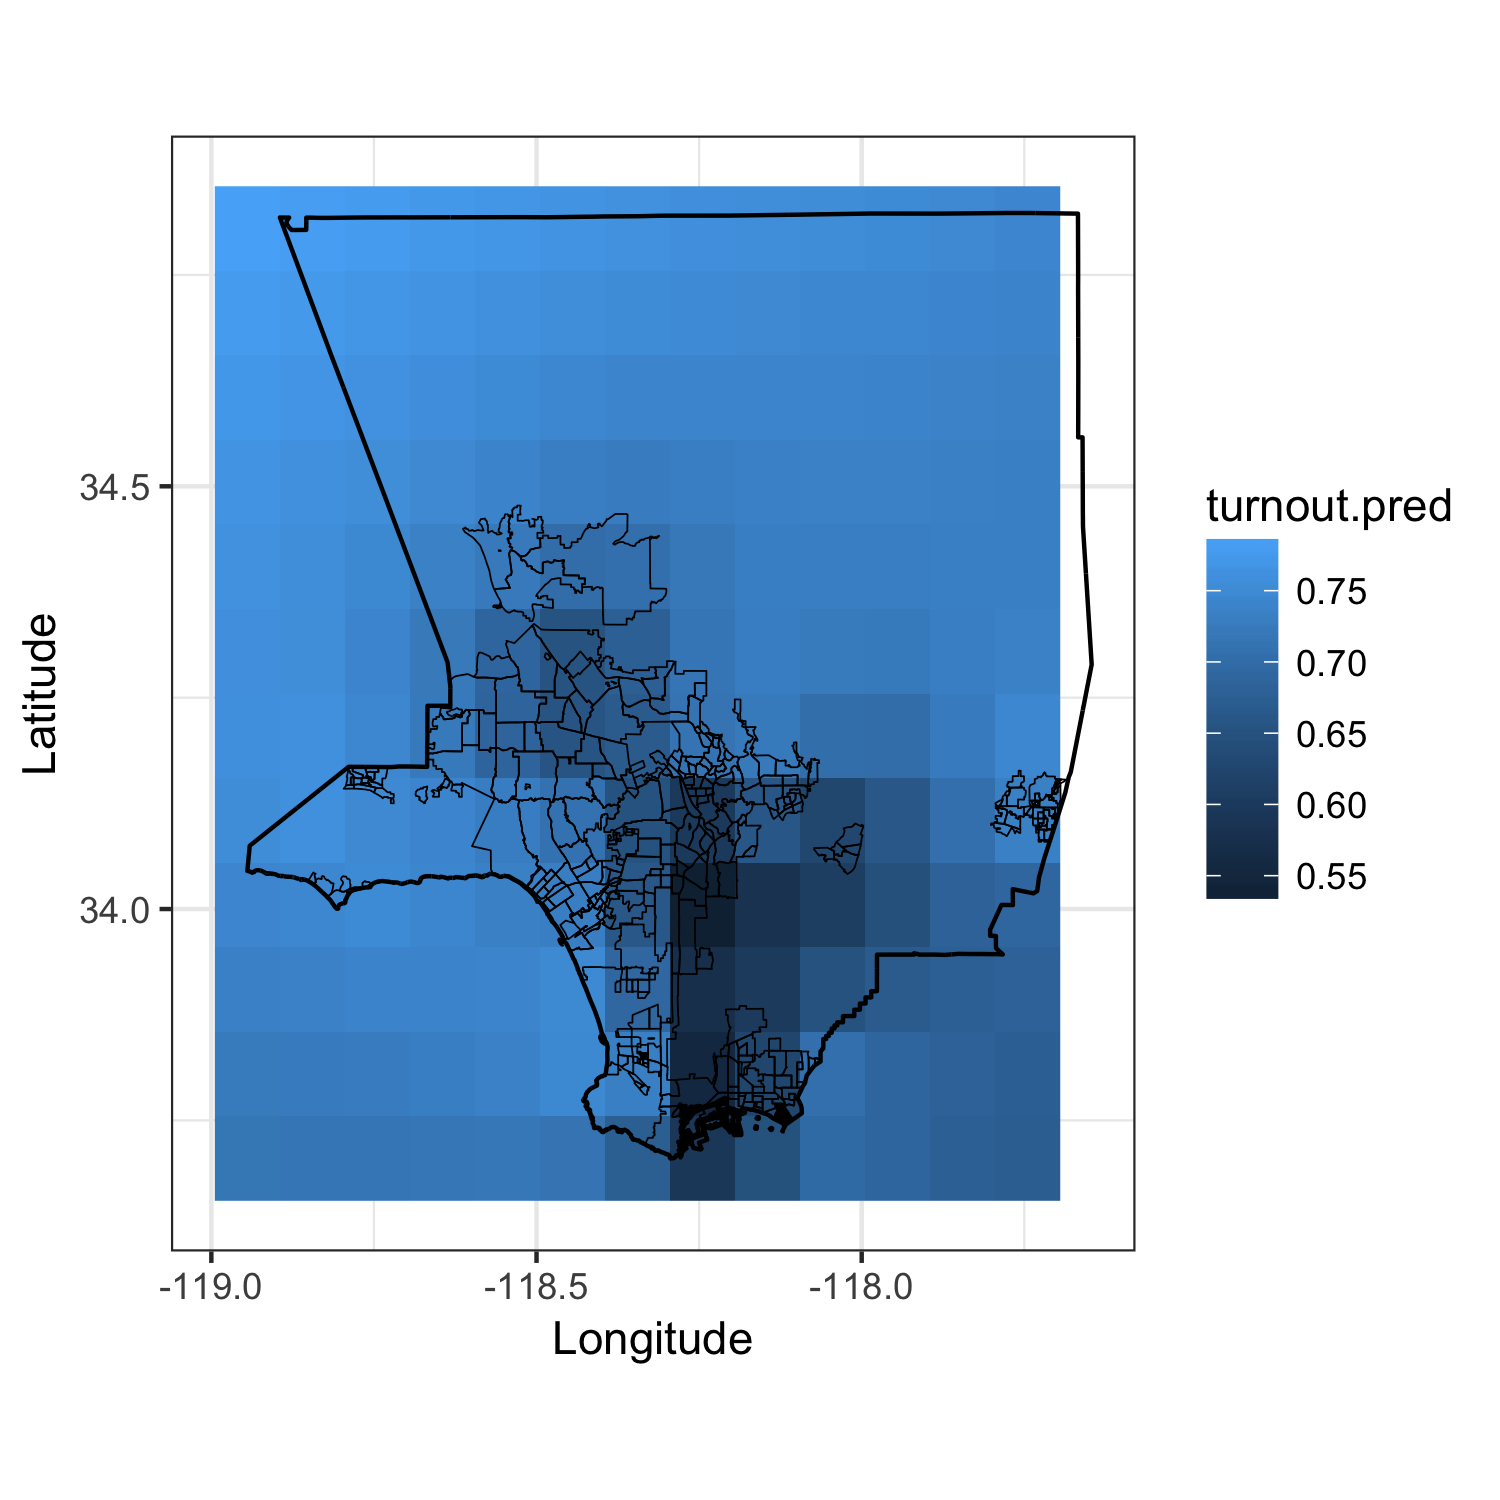
\includegraphics[width=85mm]{/Users/bryanwilcox/Dropbox/Courses/UCLA/2017_winter/stats_273_geostats/stats_273_geo_stats/pred_uk.png}\\  
%\vskip-6ex
\end{figure} 
\end{frame}

\begin{frame}{Next Steps}
\begin{itemize}
\item Try to obtain precincts instead of neighborhood (maybe zipcodes).
\pause
\item Try to obtain polling locations and look at how spatial variation between polling location distance. 
\pause
\end{itemize}

Question, comments, other thoughts? 
\end{frame}




\end{document}


{ % all template changes are local to this group.
    \setbeamertemplate{navigation symbols}{}
    \begin{frame}
    %\frametitle{Restaurants, Stores, Signs, and Murals}
        \begin{tikzpicture}[remember picture,overlay]
            \node[at=(current page.center)] {
                \includegraphics[width=\paperwidth, height=\paperheight]{DSC_0466.JPG}
            };
        \end{tikzpicture}
     \end{frame}
}

